\documentclass[11pt]{article}
\usepackage[margin=1in]{geometry}

\usepackage{amsmath}
\usepackage{amssymb}
\usepackage[utf8]{inputenc} 
\usepackage{graphicx} 
\usepackage{parskip} 
\usepackage{multirow} 
\usepackage{mathtools}

\DeclarePairedDelimiter\abs{\lvert}{\rvert}%
\DeclarePairedDelimiter\norm{\lVert}{\rVert}%

\makeatletter
\let\oldabs\abs
\def\abs{\@ifstar{\oldabs}{\oldabs*}}

\let\oldnorm\norm
\def\norm{\@ifstar{\oldnorm}{\oldnorm*}}
\makeatother
\usepackage{multicol} 
\usepackage[spanish,es-nodecimaldot]{babel} 
\usepackage{mathtools}
\usepackage{amsfonts}
\usepackage{float}
\usepackage{textcomp}
\usepackage{caption}
\usepackage{subfig}
\usepackage[spanish]{babel}
\usepackage{gensymb}
\def\sen{\mathop{\mbox{\normalfont sen}}\nolimits}

\usepackage{fancyhdr}
\fancyhf{}
\rfoot{\thepage}
\pagestyle{fancy}
\lhead{Nieto Castellanos Jaime Fabián}
\chead{}
\rhead{Tarea 7. Histogramas}
\begin{document}

\textbf{1)}
\begin{figure}[H]
\centering
\subfloat[\centering Curva de calibración para el tanque 96, pulsos pequeños]{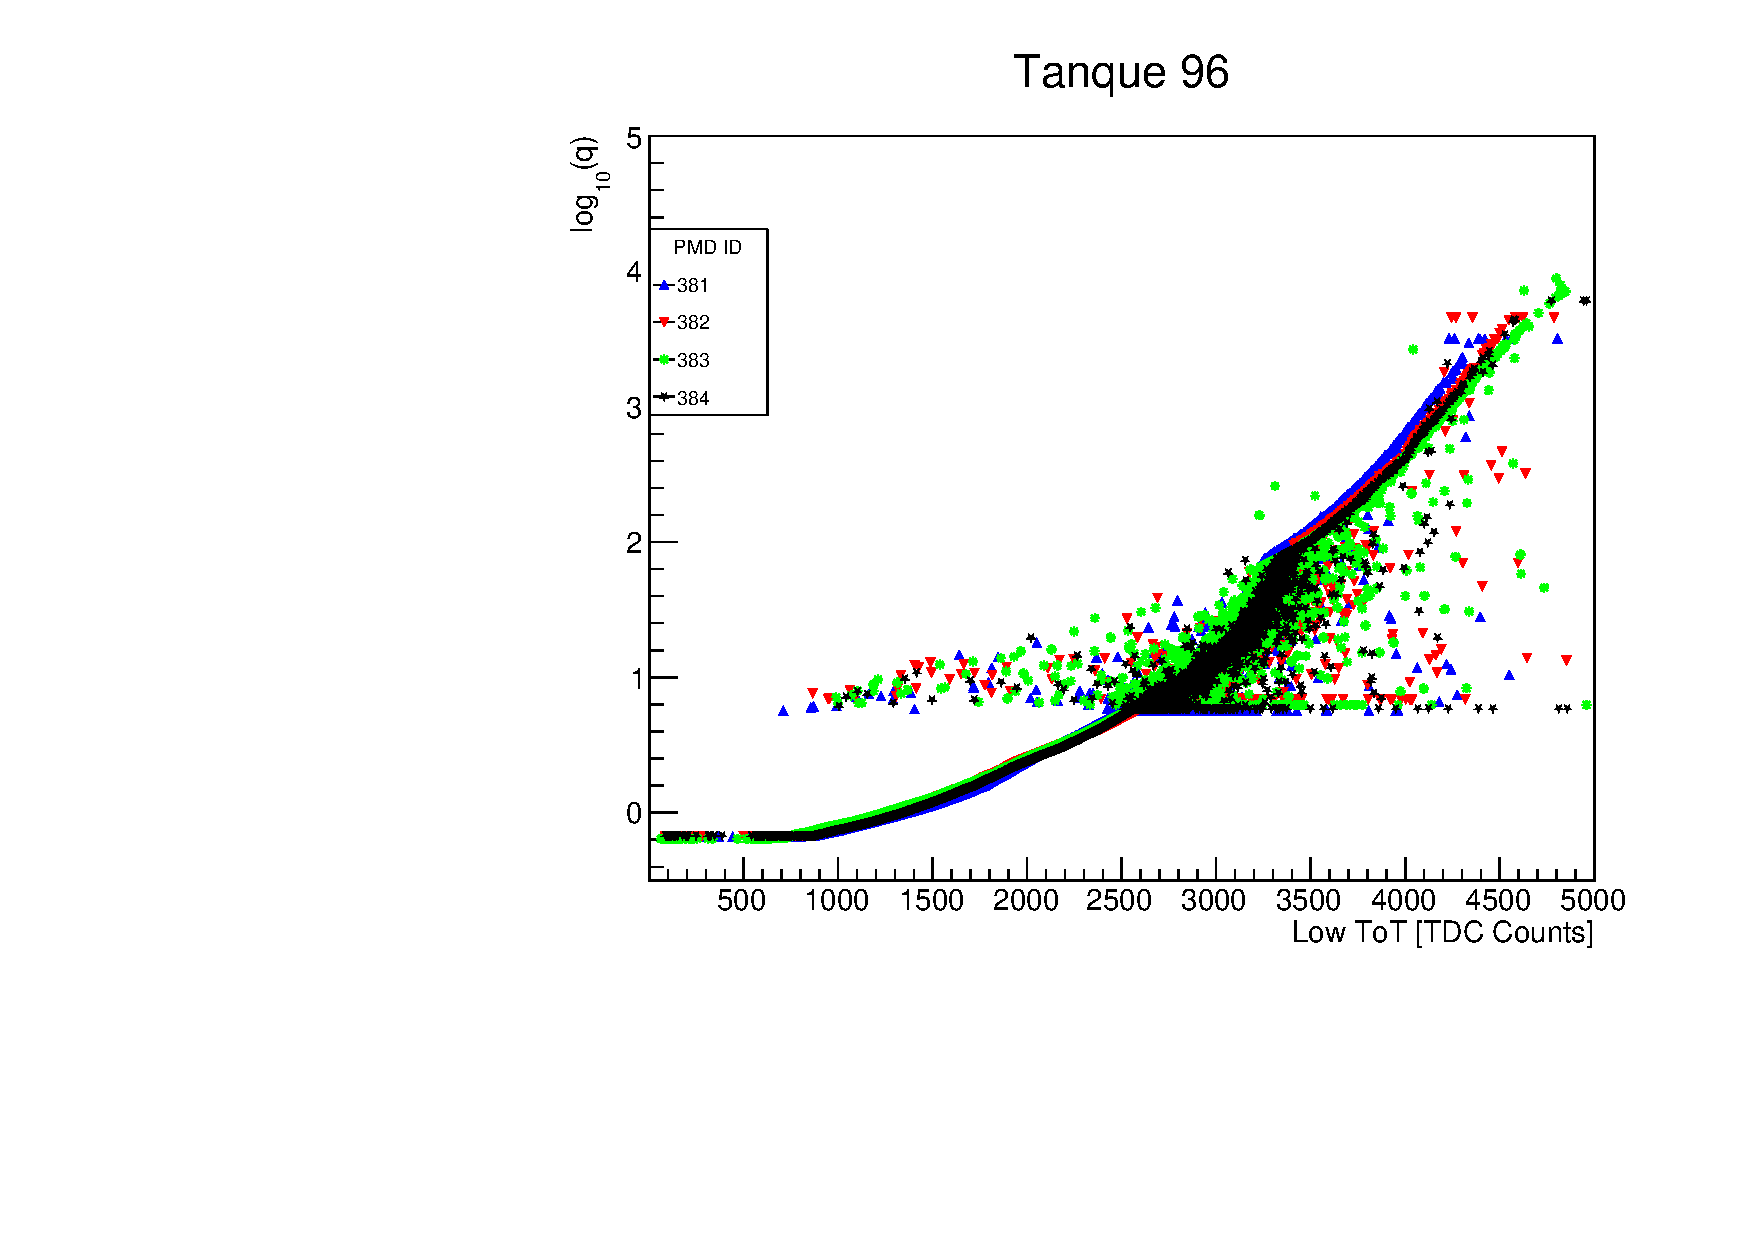
\includegraphics[width=0.7\textwidth]{../Figuras/Prob1A.pdf}}

\subfloat[\centering Curva de calibración para el tanque 96, pulsos grandes]{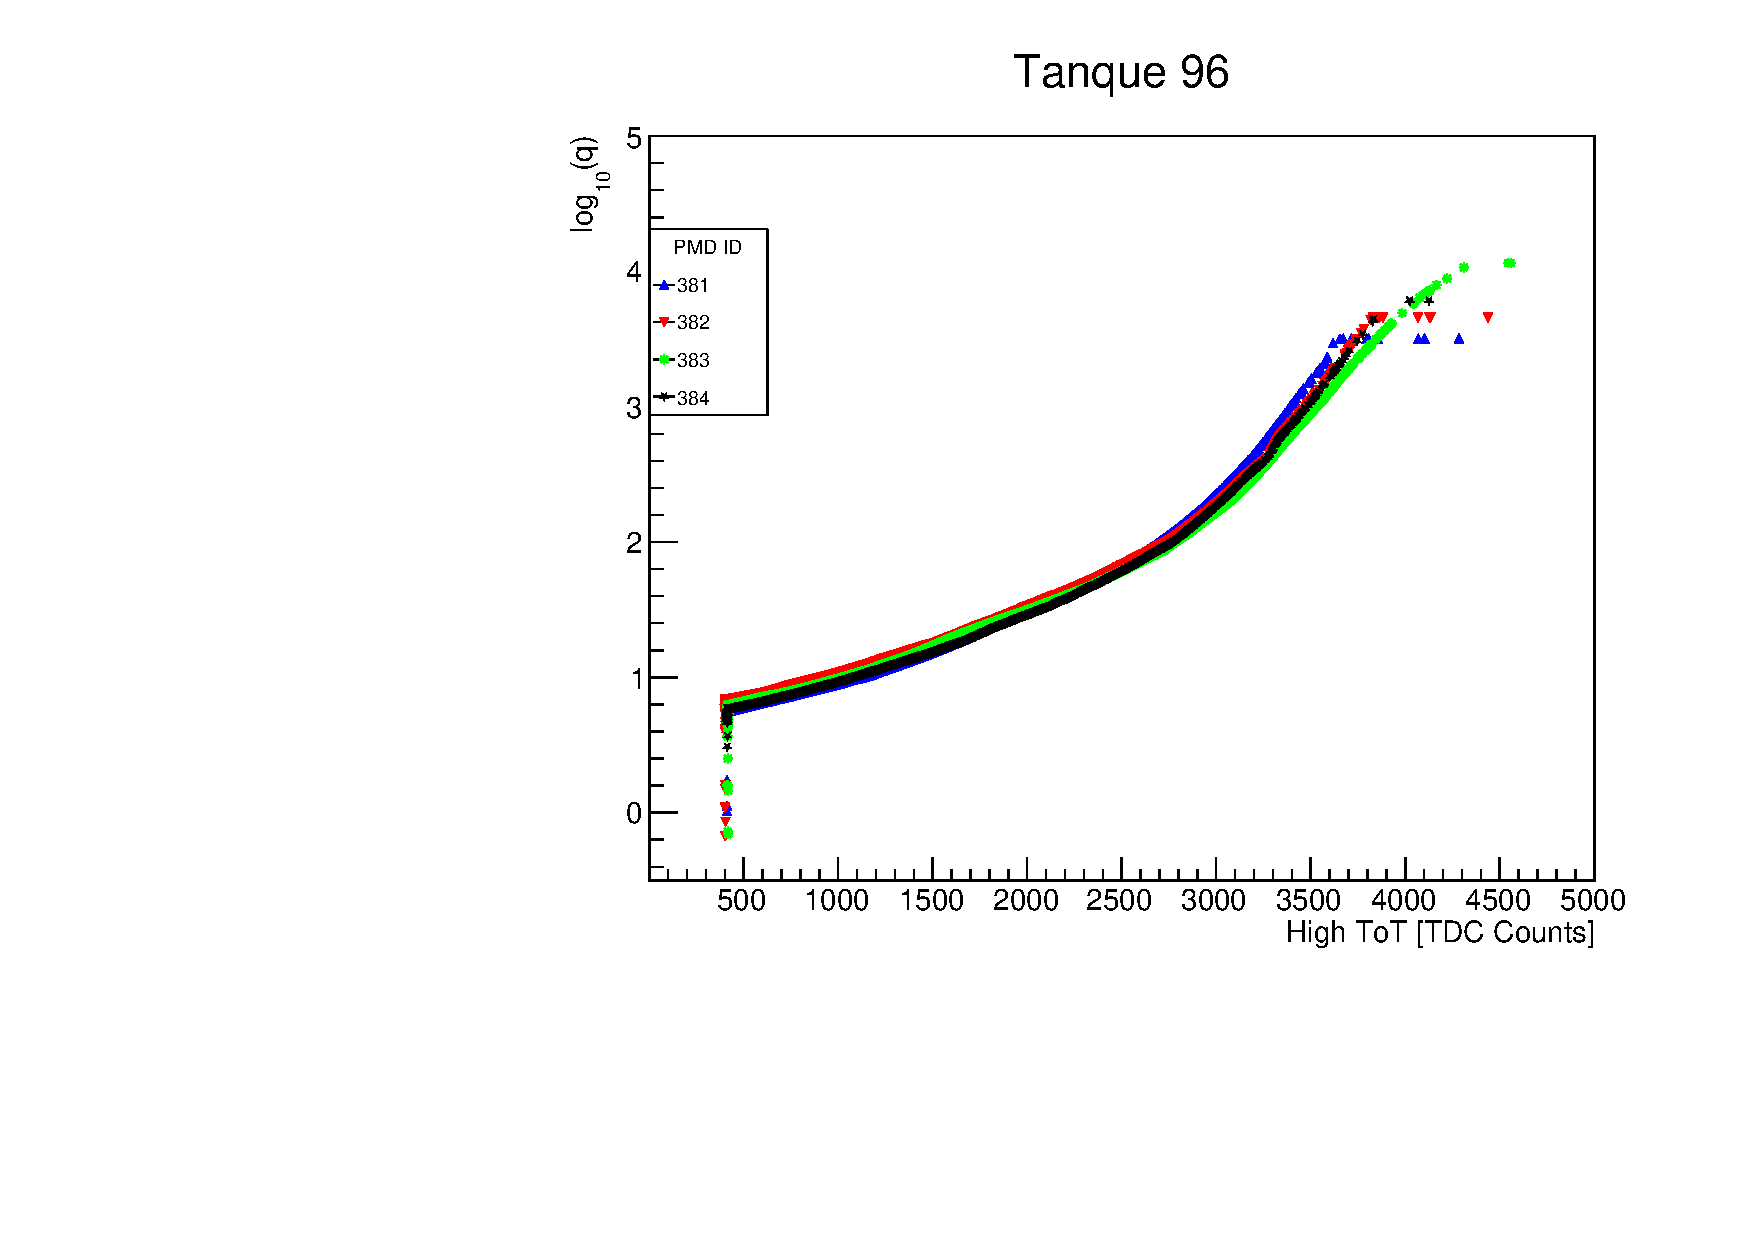
\includegraphics[width=0.7\textwidth]{../Figuras/Prob1B.pdf}}
\caption{Curva de calibración de los PMTs correspondientes al tanque número 96}
\label{fig:Prob1}
\end{figure}
\pagebreak
%%%%%%%%%%%%%%%%%%%%%%%%%%%%%%%%%%%%%%%%%%%%%%%%
\textbf{2)}
\begin{figure}[H]
\centering
\subfloat[\centering Curva de calibración para el PMT central del tanque 96 (PMT ID 383) y para el PMT central del tanque 291 (PMT ID 1163) pulsos pequeños]{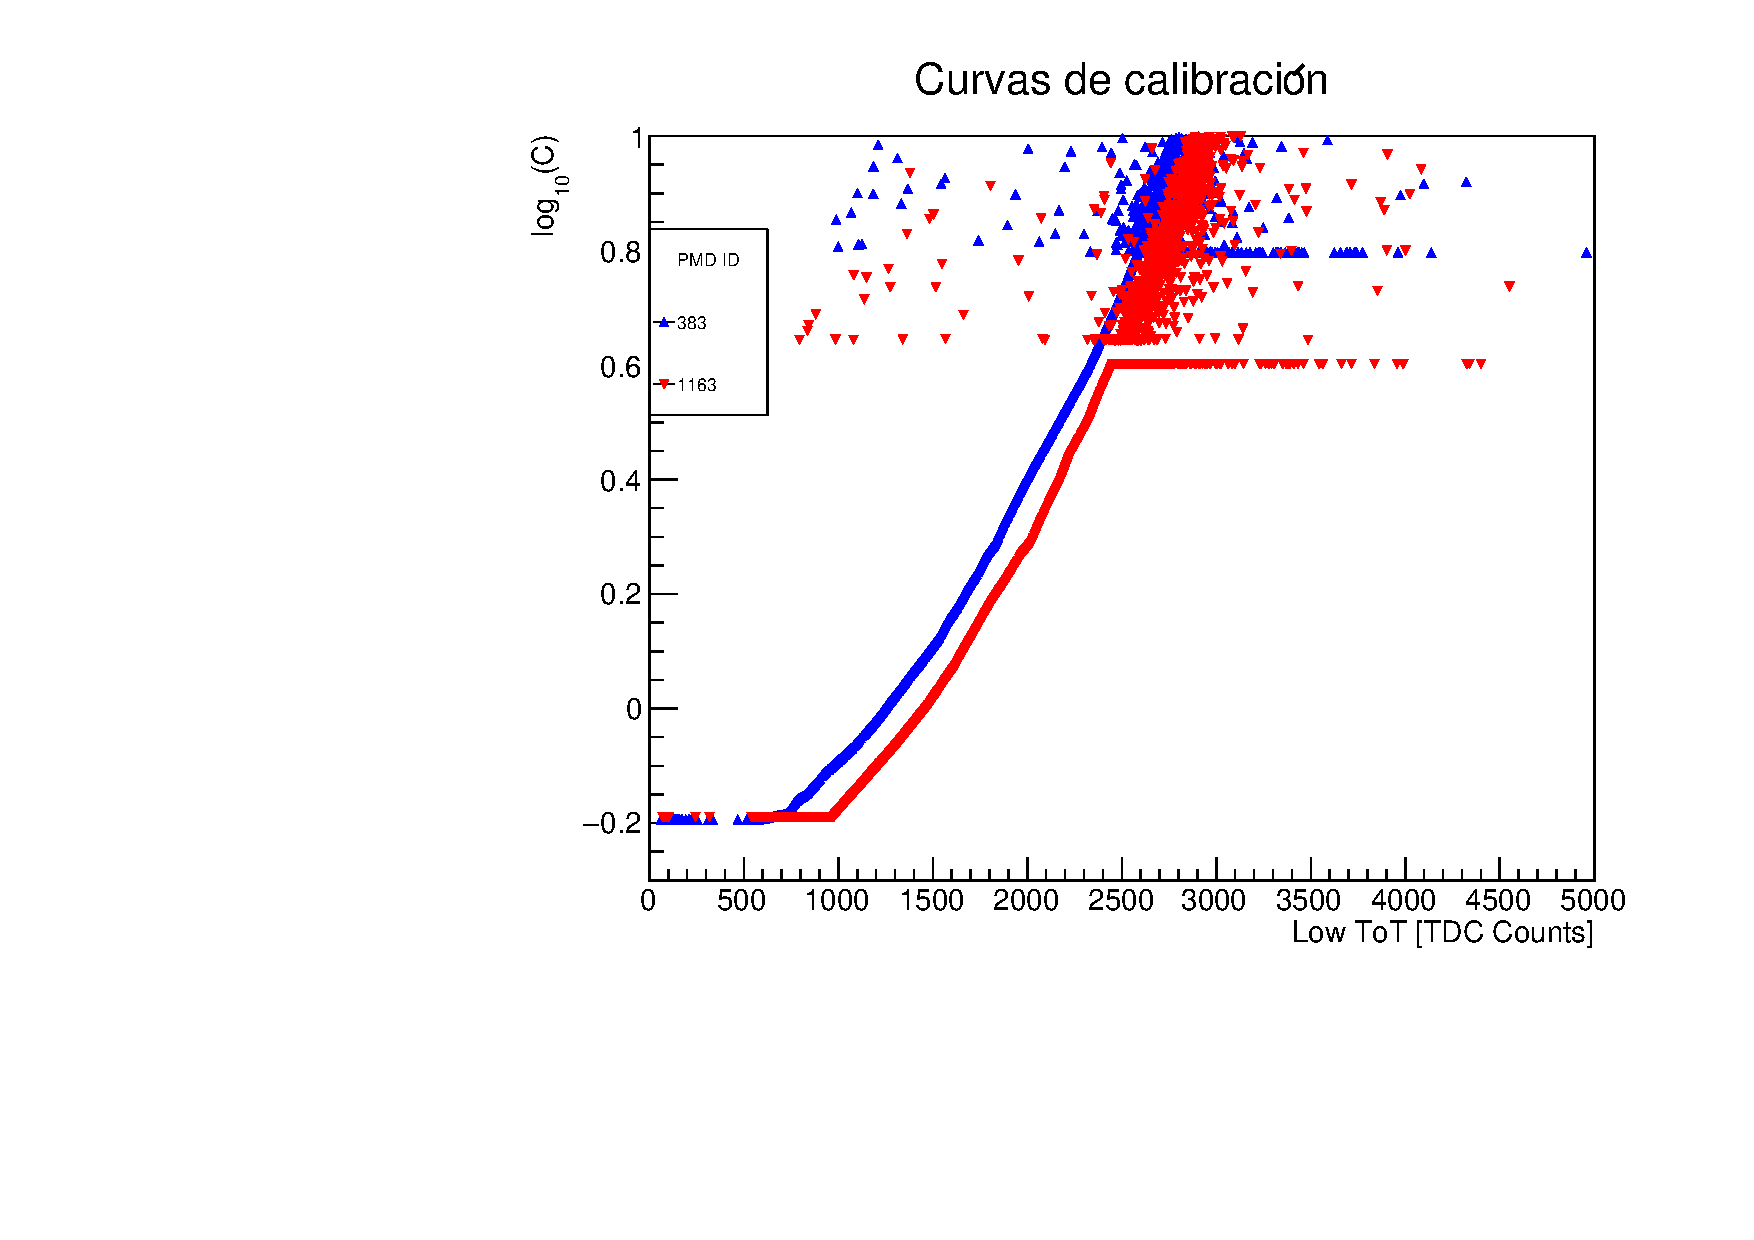
\includegraphics[width=0.7\textwidth]{../Figuras/Prob2A.pdf}}

\subfloat[\centering Curva de calibración para el PMT central del tanque 96 (PMT ID 383) y para el PMT central del tanque 291 (PMT ID 1163), pulsos grandes]{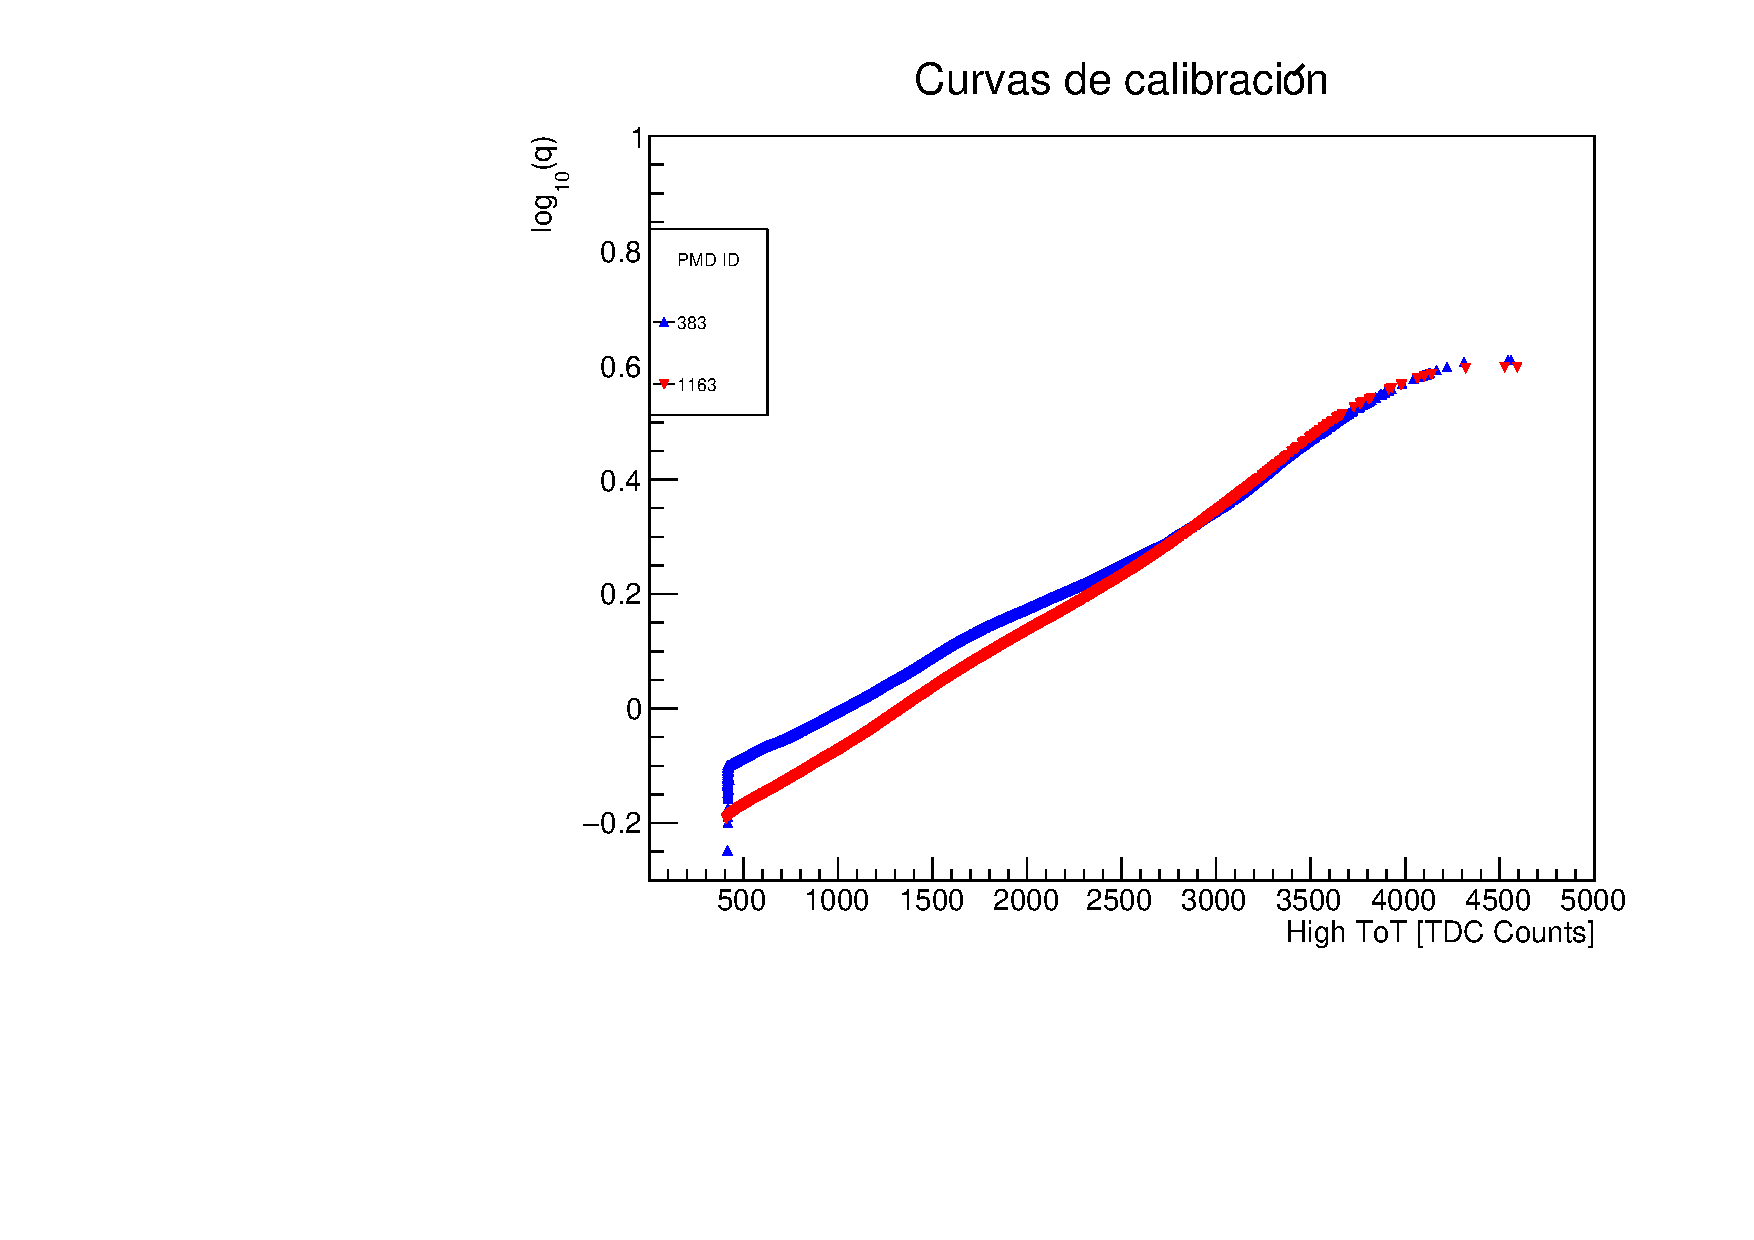
\includegraphics[width=0.7\textwidth]{../Figuras/Prob2B.pdf}}
\caption{Curva de calibración de los PMTs correspondientes a dos PMT's centrales}
\label{fig:Prob2}
\end{figure}
Las curvas son similares para dos PMT's centrales, sin embargo no son exactamente iguales, pues para el PMT del tanque 291 la carga es menor cuando el número de cuentas asociadas a pulsos grandes es menor a 2,500.
\pagebreak

%%%%%%%%%%%%%%%%%%%%%%%%%%%%%%%%%%%%%%%%%%%%%%%%
\textbf{3)}
\begin{figure}[H]
\centering
\subfloat[\centering Curva de calibración para los PMT's del tanque 96 usando la carga efectiva, pulsos pequeños]{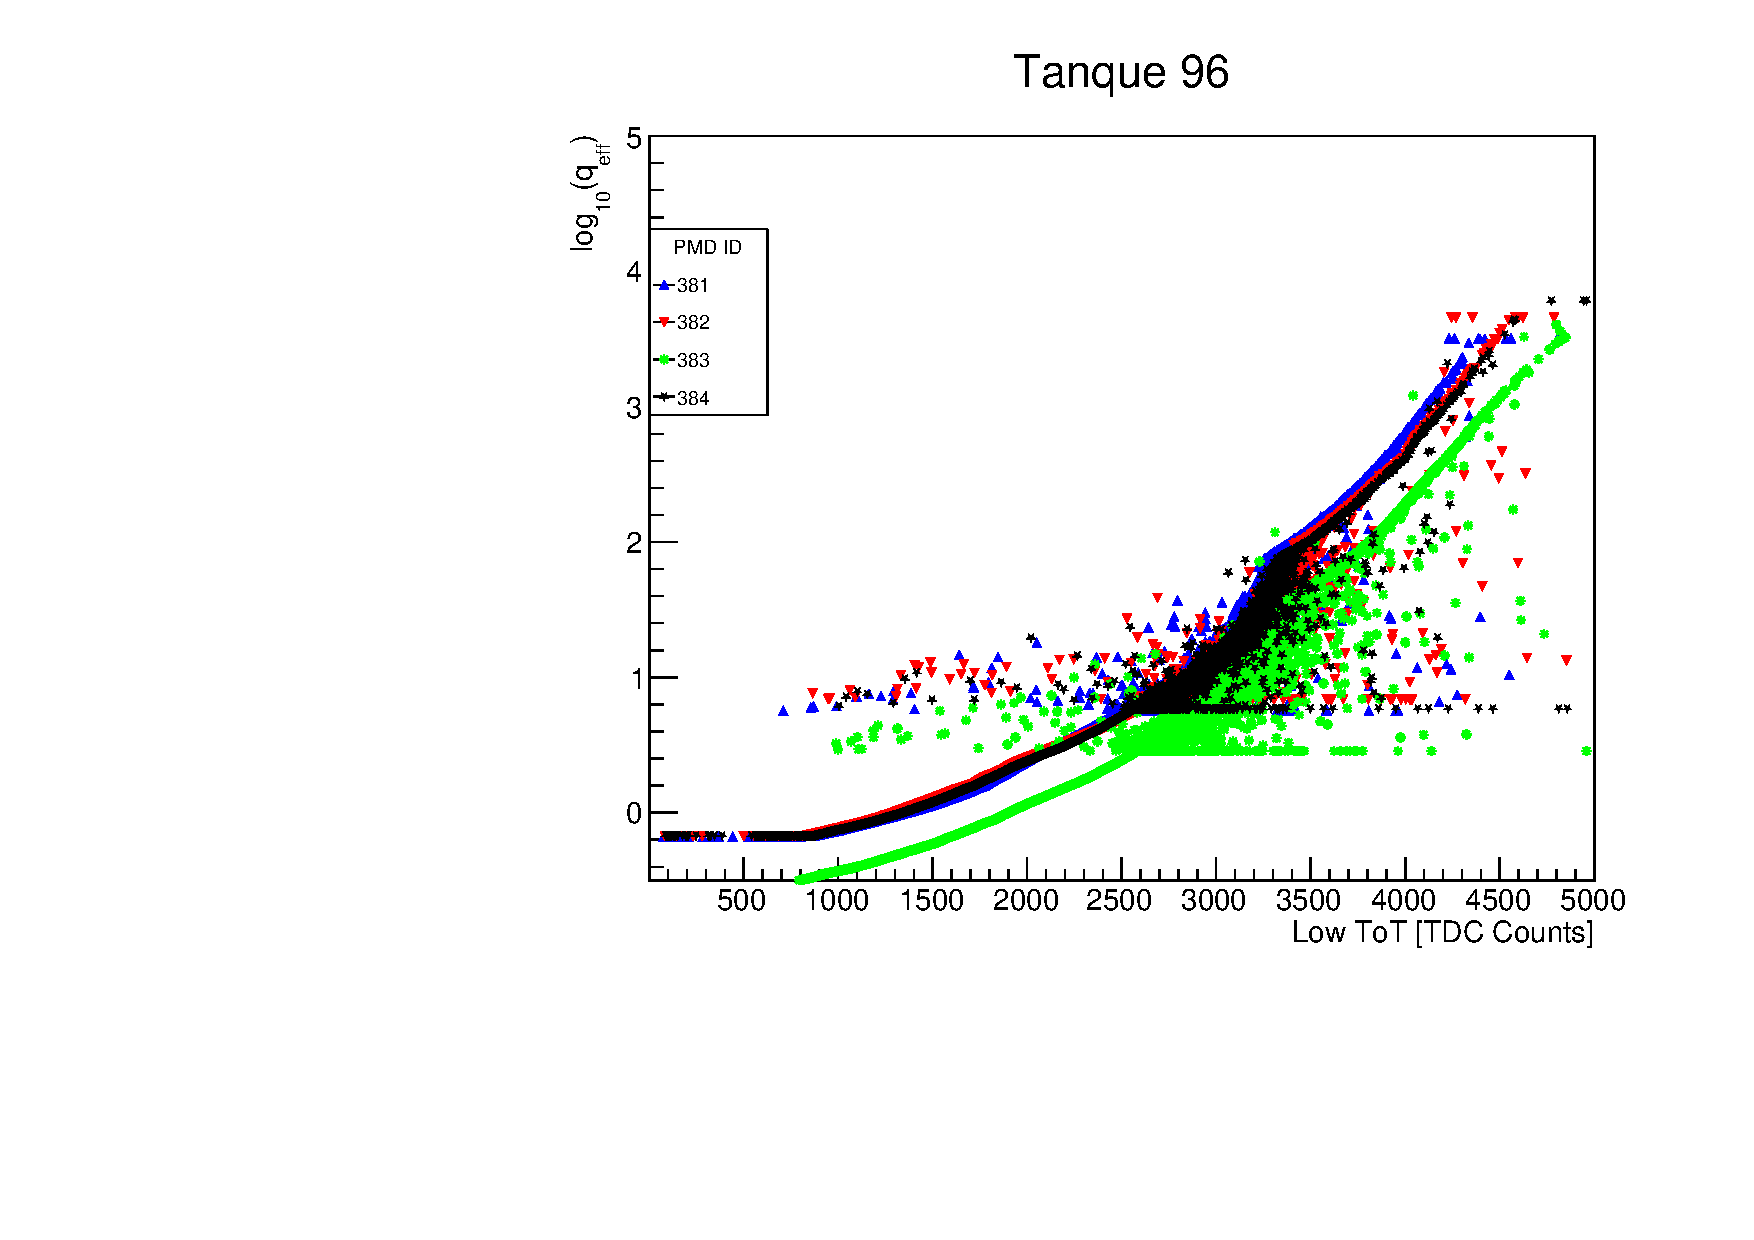
\includegraphics[width=0.7\textwidth]{../Figuras/Prob3A.pdf}}

\subfloat[\centering Curva de calibración para los PMT's del tanque 96 usando la carga efectiva, pulsos grandes]{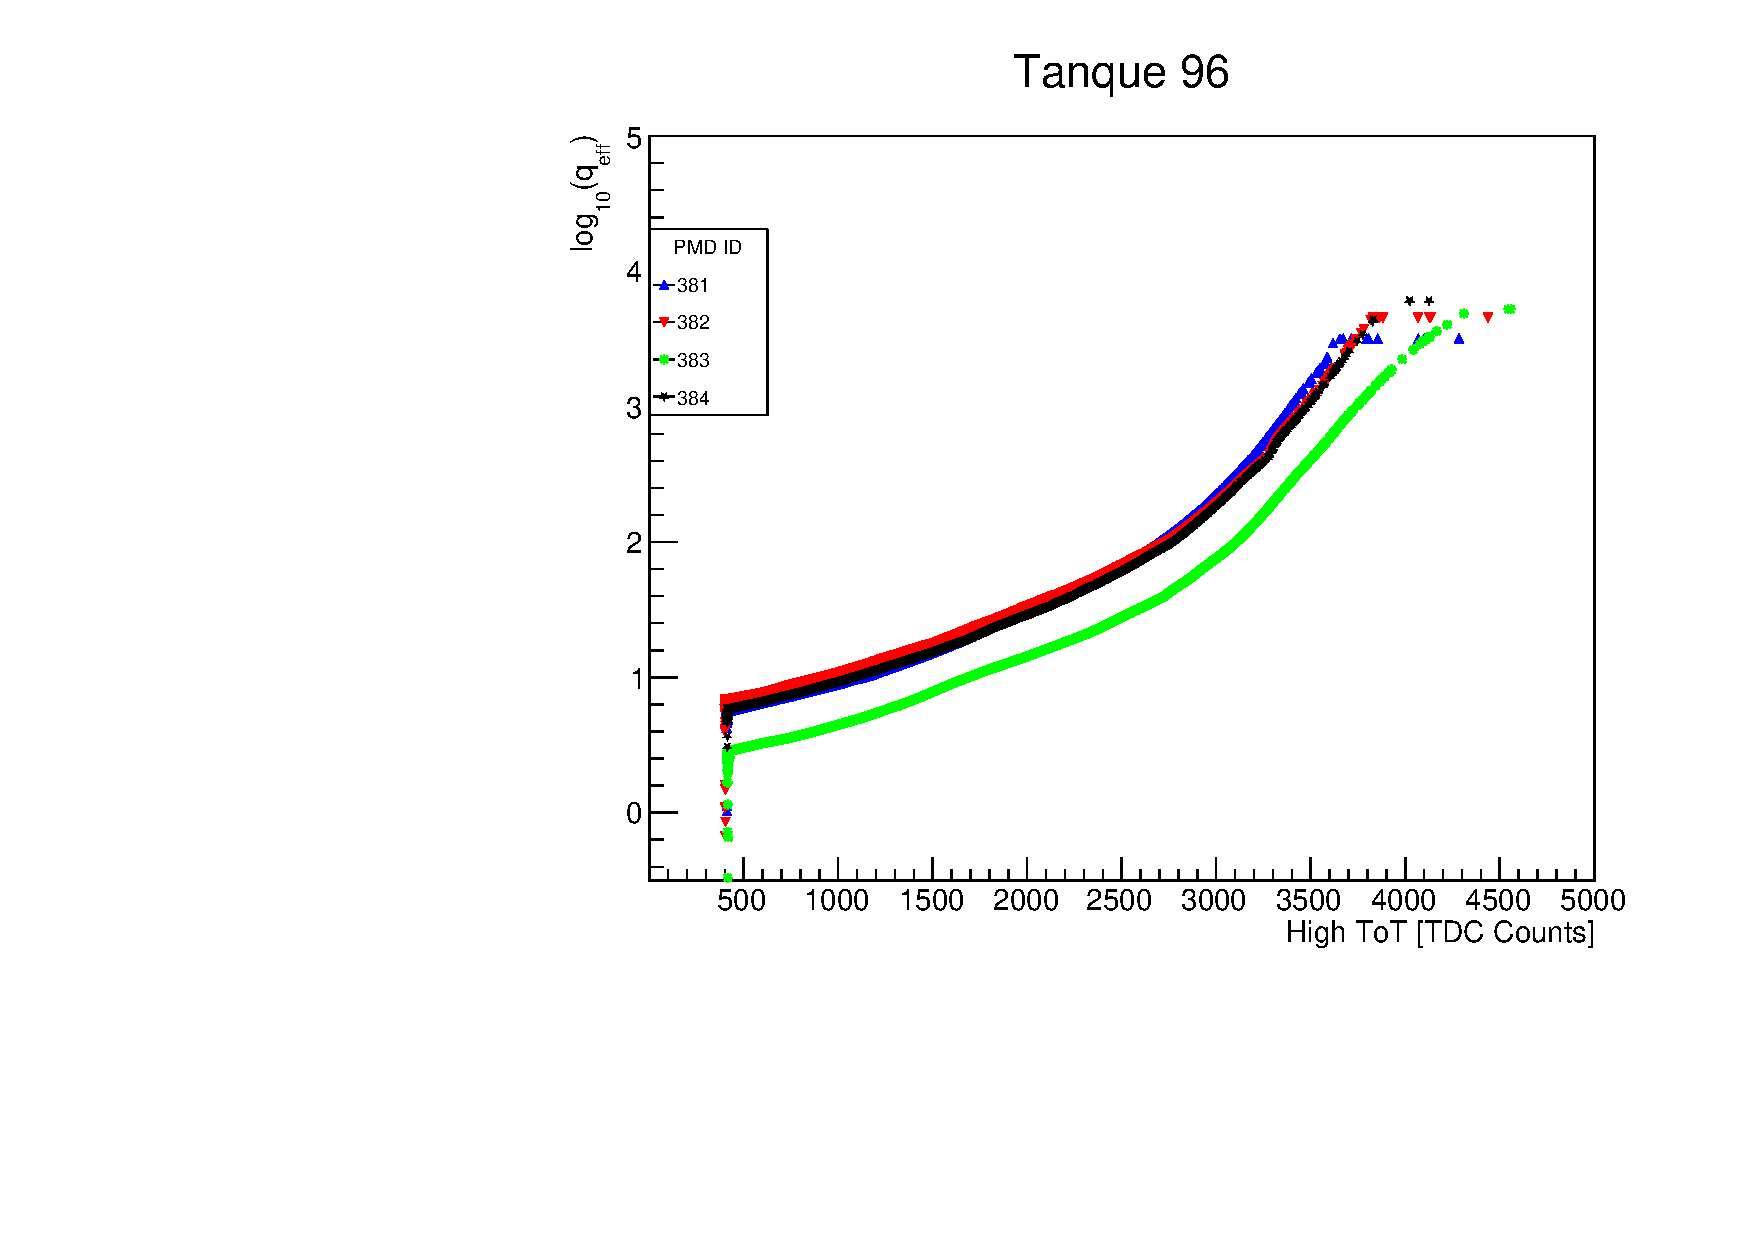
\includegraphics[width=0.7\textwidth]{../Figuras/Prob3B.pdf}}
\end{figure}

\begin{figure}[H]
\centering
\subfloat[\centering Comparación entre la carga efectiva y la carga calibrada]{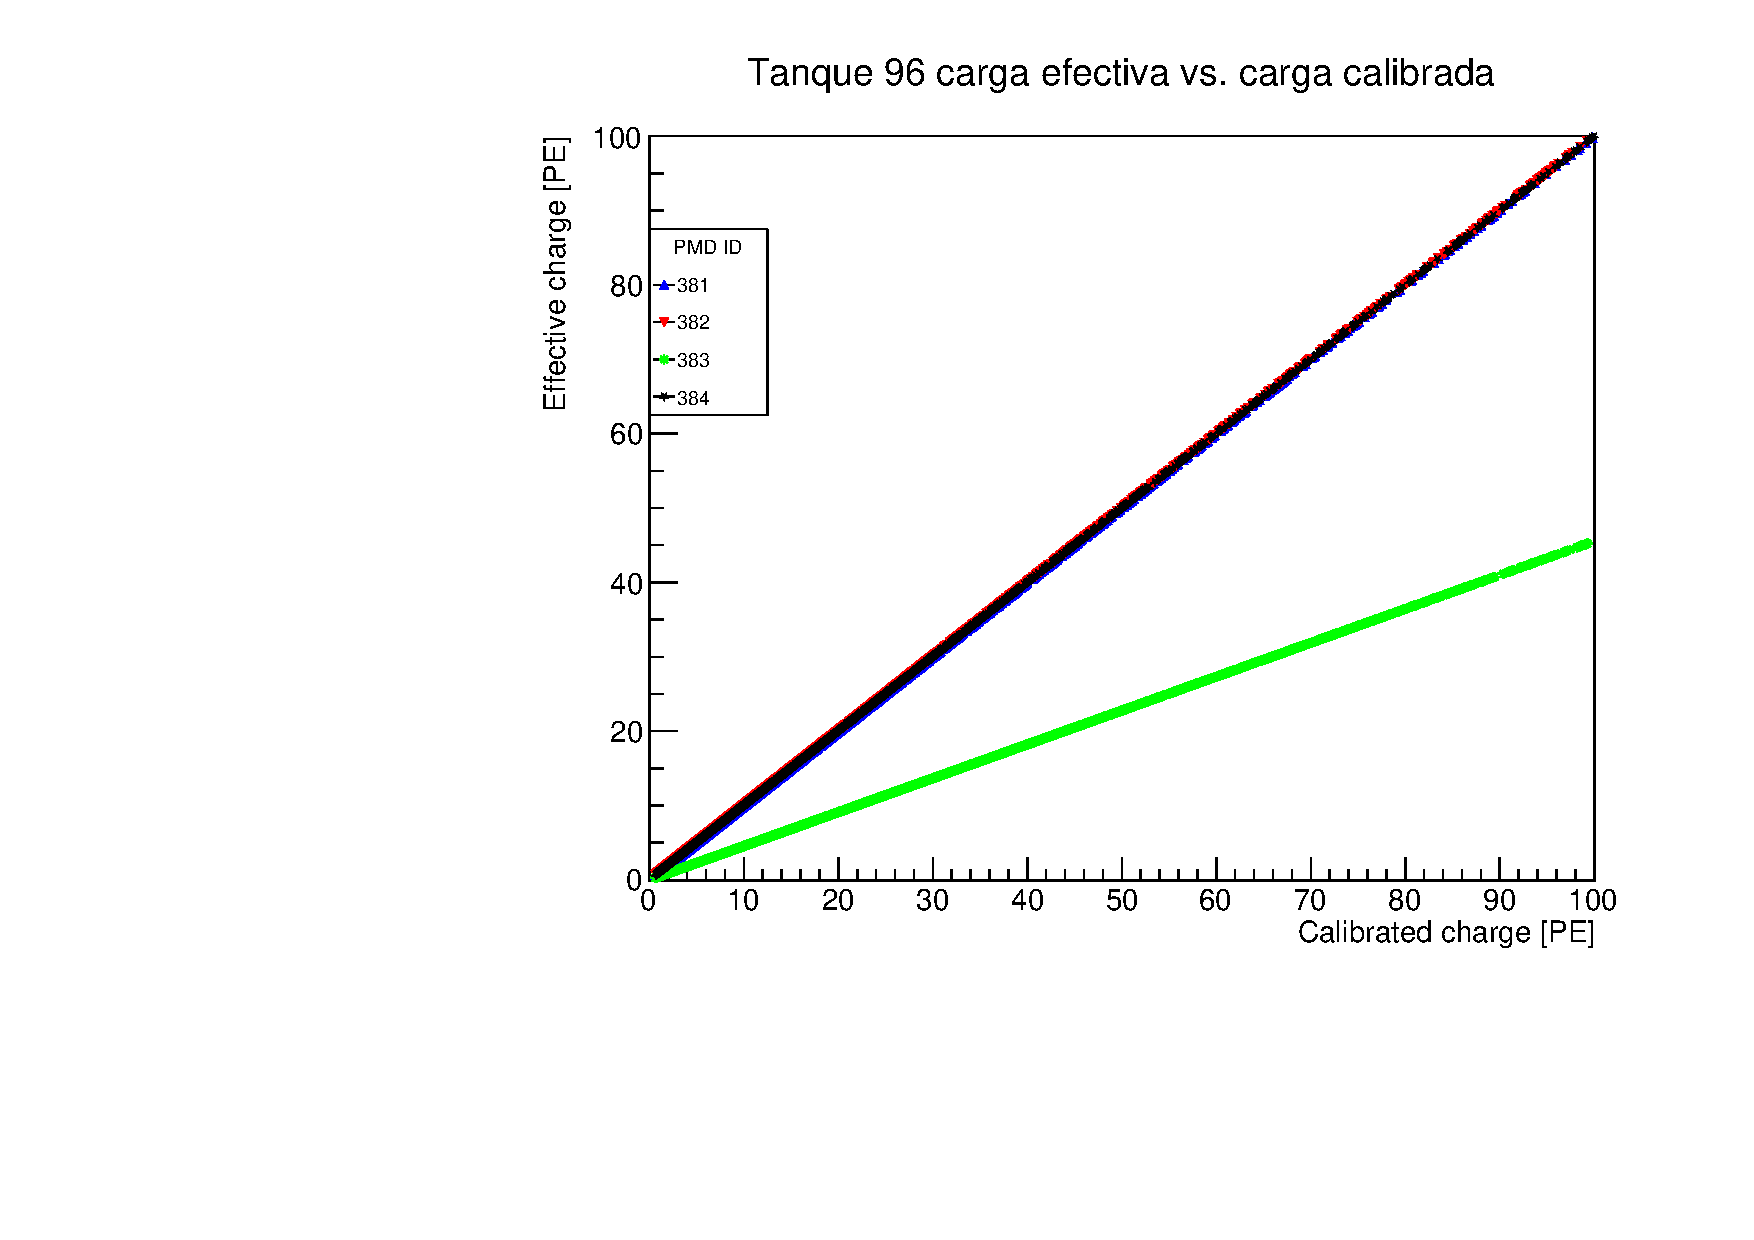
\includegraphics[width=0.7\textwidth]{../Figuras/Prob3C.pdf}}
\caption{Comparación del análisis previo usando la carga calibrada y la carga efectiva.}
\label{fig:Prob3}
\end{figure}


Se observa que el resultado es igual para 3 PMT's, independientemente de qué carga utilicemos. Sin embargo, para el PMT central la carga efectiva es menor que la carga calibrada, aunque la relación entre estas sigue siendo lineal. Esto sugiere que la carga efectiva y la carga calibrada son iguales a excepción del PMT central. 
\pagebreak

\textbf{4)}

\textbf{a), b), c) y d)}

Para este ejercicio elegimos las cascadas atmosféricas que corresponden al evento número 10, al 724 y al 3. El máximo número de hits que puede tener un evento del archivo de datos es 1860, por lo que diremos que un evento es chico si tiene menos de 1860/3 = 620 hits, es mediano cuando su número de hits es mayor a 620 y menor a 1240 y es grande cuando el número de hits es mayor a 1240.

\hspace{5mm}El evento 10 tiene 1054 hits (evento mediano), el evento 724 tiene 564 hits (evento pequeño) y el evento 3 tiene 1275 hits (evento grande). Se usaron dos criterios para hacer el corte de calidad. Primero, se verificó que la señal de los PMT fuese buena, es decir, que la variable channelIsGood fuese igual a 1. El otro criterio usado consistió en revisar que la variable stdCuts.isSelected también sea igual a 1 para verificar que se satisfacen cortes estándar.

\hspace{5mm}Finalmente, de las funciones que se trataron de ajustar, una de la forma $a\,\textrm{exp}(-bx)$ resultó más exitosa. En la figura \ref{fig:Prob4} se muestran los resultados.

\begin{figure}[H]
\centering

\subfloat[\centering Distribución lateral de un evento mediano. Los parámetros del ajuste dados por root son $a=3.107(30)$, $b=-0.0236(3)$]{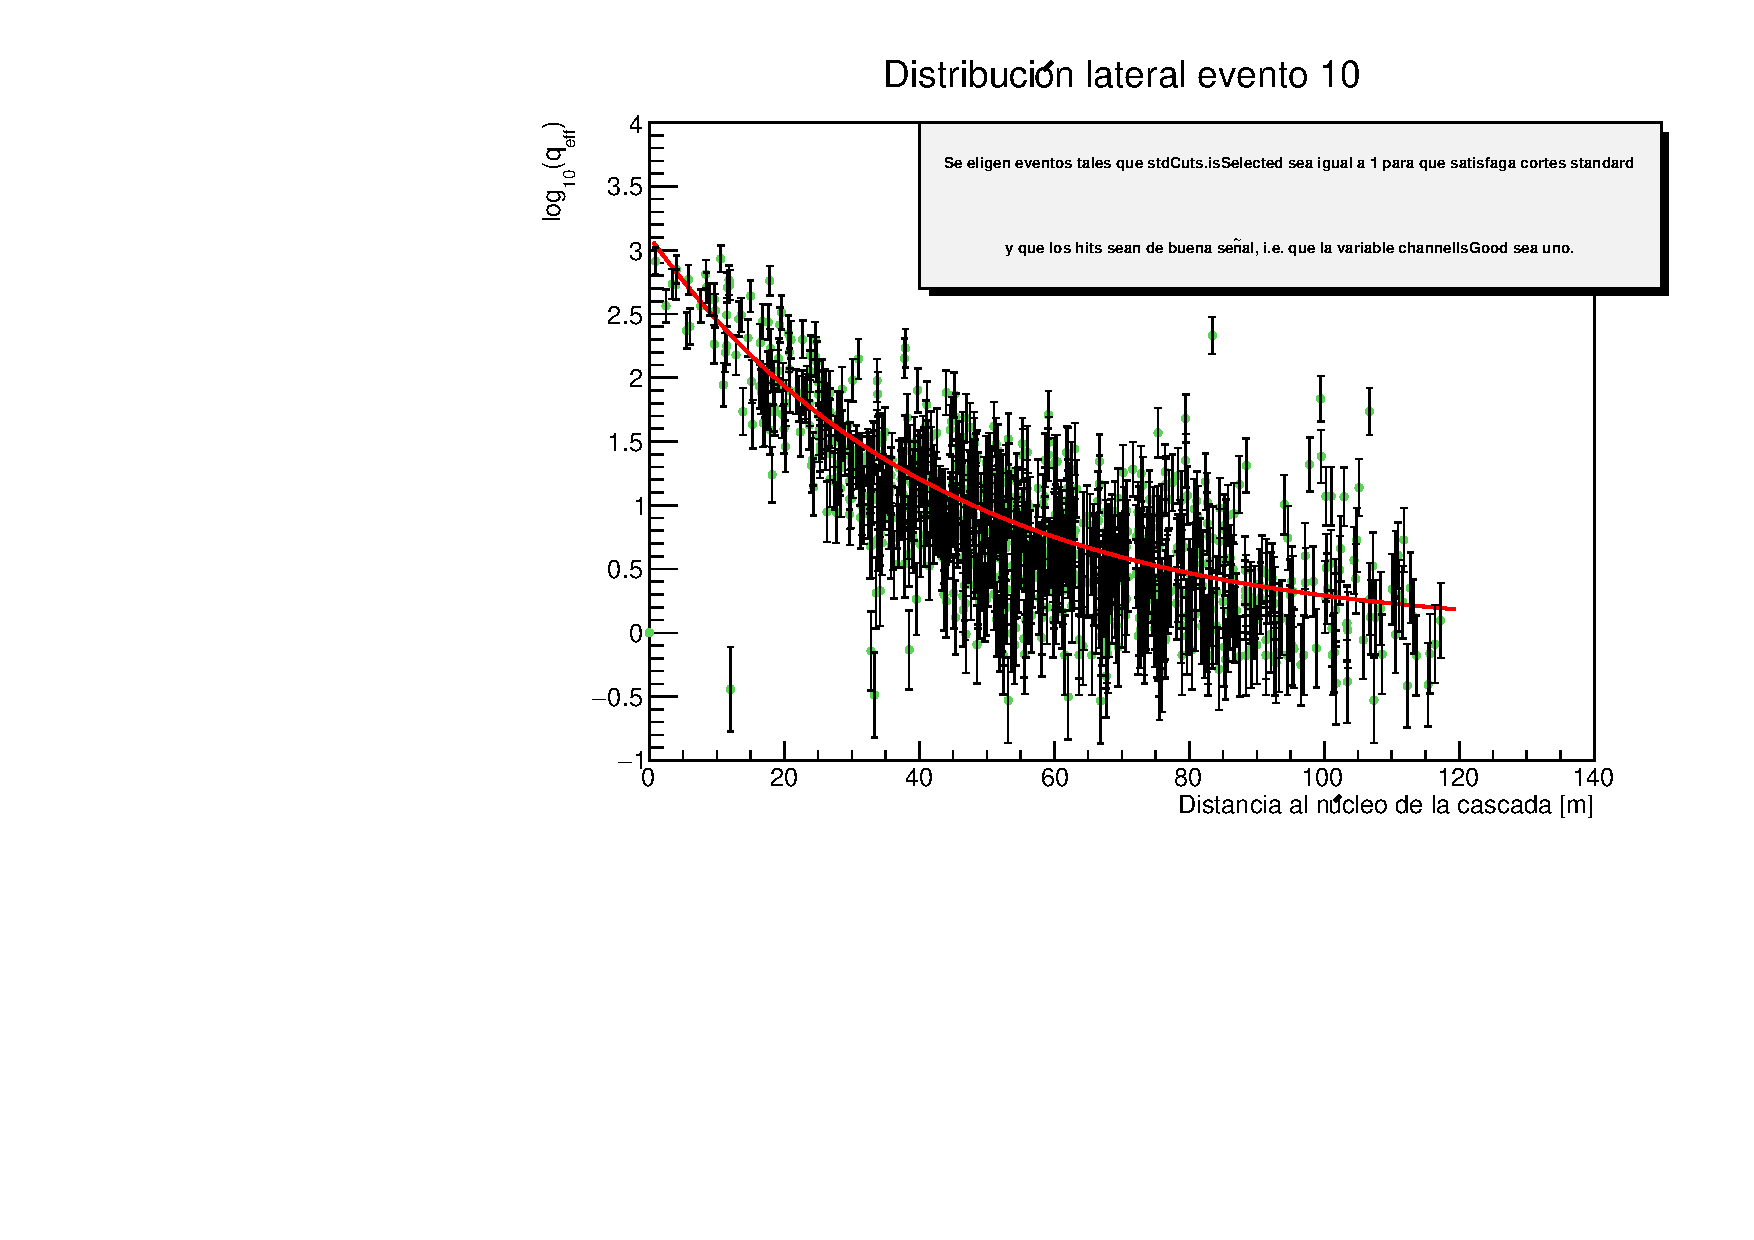
\includegraphics[width=0.9 \textwidth]{../Figuras/Prob4A.pdf}}

\subfloat[\centering Distribución lateral de un evento pequeño. Los parámetros del ajuste dados por root son $a=3.083(39)$, $b=-0.0243(5)$]{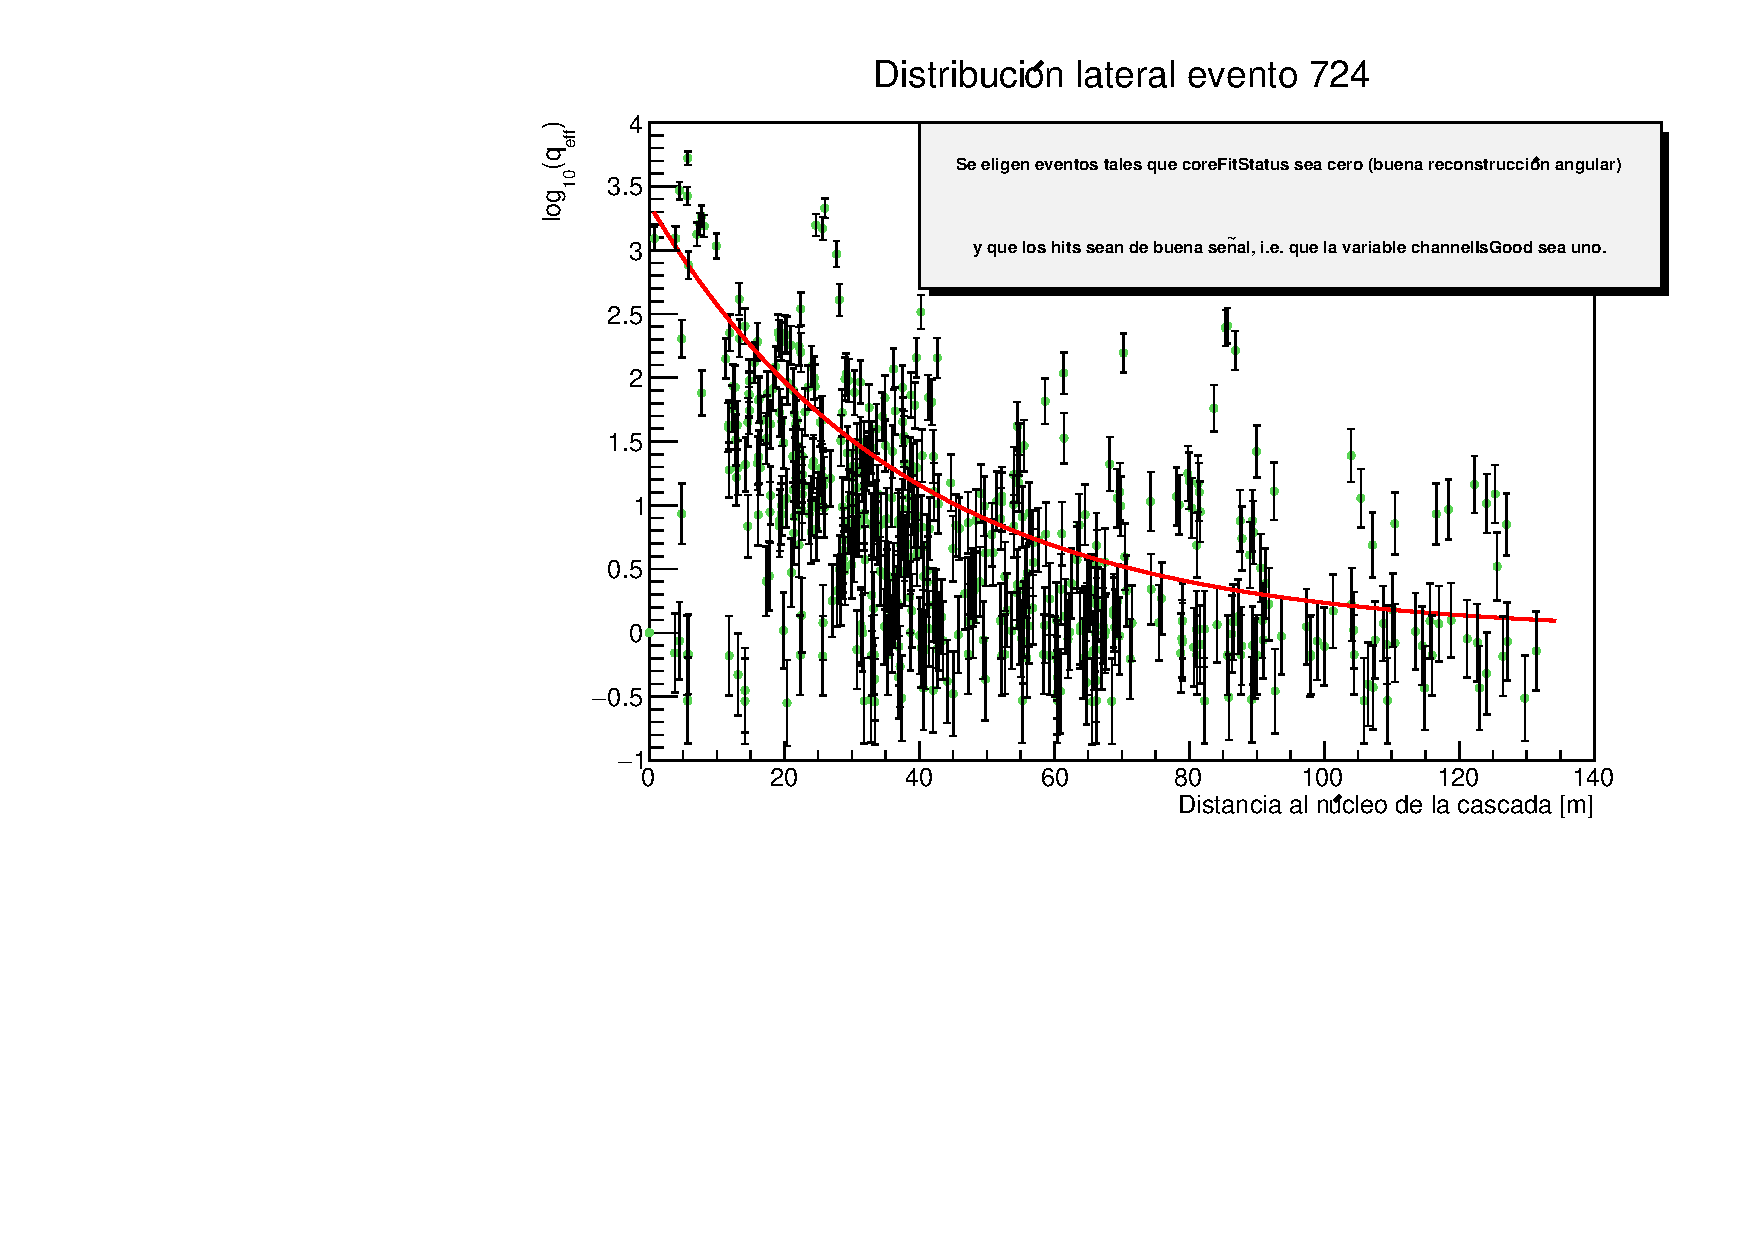
\includegraphics[width=0.9 \textwidth]{../Figuras/Prob4B.pdf}}
\end{figure}

\begin{figure}[H]
\subfloat[\centering Distribución lateral de un evento pequeño. Los parámetros del ajuste dados por root son $a=3.123(19)$, $b=-0.00510(7)$]{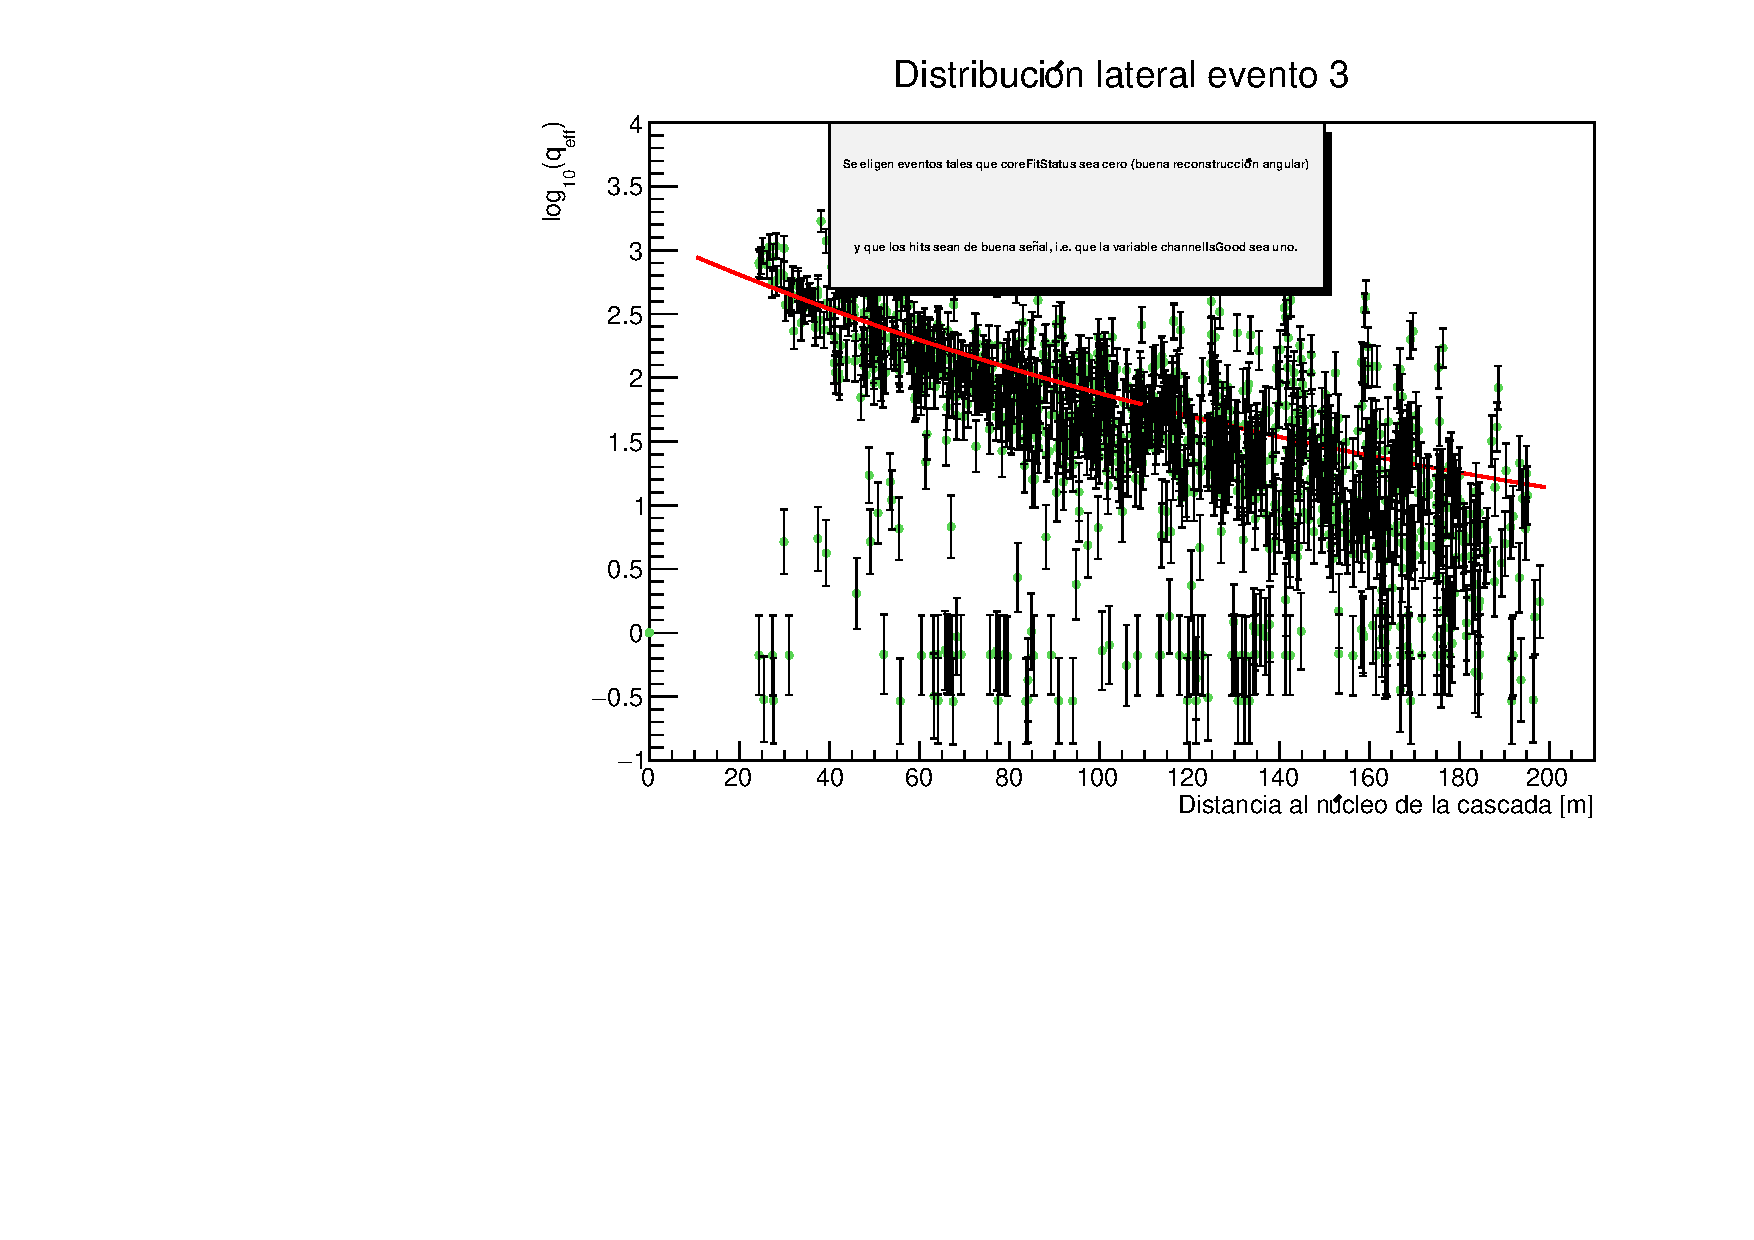
\includegraphics[width=0.9 \textwidth]{../Figuras/Prob4C.pdf}}
\caption{Distribución lateral de tres eventos distintos. Se ajustó una función de la forma $a\,\textrm{exp}(-bx)$}
\label{fig:Prob4}
\end{figure}



\end{document}